
%%%%%%%%%%%%%%%%%%%%%%% file typeinst.tex %%%%%%%%%%%%%%%%%%%%%%%%%
%
% This is the LaTeX source for the instructions to authors using
% the LaTeX document class 'llncs.cls' for contributions to
% the Lecture Notes in Computer Sciences series.
% http://www.springer.com/lncs       Springer Heidelberg 2006/05/04
%
% It may be used as a template for your own input - copy it
% to a new file with a new name and use it as the basis
% for your article.
%
% NB: the document class 'llncs' has its own and detailed documentation, see
% ftp://ftp.springer.de/data/pubftp/pub/tex/latex/llncs/latex2e/llncsdoc.pdf
%
%%%%%%%%%%%%%%%%%%%%%%%%%%%%%%%%%%%%%%%%%%%%%%%%%%%%%%%%%%%%%%%%%%%


\documentclass[runningheads,a4paper]{llncs}

\usepackage{amssymb}
\setcounter{tocdepth}{3}
\usepackage{graphicx}

\usepackage{url}
\usepackage{todonotes}
\urldef{\mailsa}\path|{alfred.hofmann, ursula.barth, ingrid.haas, frank.holzwarth,|
\urldef{\mailsb}\path|anna.kramer, leonie.kunz, christine.reiss, nicole.sator,|
\urldef{\mailsc}\path|erika.siebert-cole, peter.strasser, lncs}@springer.com|    
\newcommand{\keywords}[1]{\par\addvspace\baselineskip
\noindent\keywordname\enspace\ignorespaces#1}

\begin{document}

\mainmatter  % start of an individual contribution

% first the title is needed
\title{Team Description Paper}

% a short form should be given in case it is too long for the running head
\titlerunning{Robocup at Work is Awesome}

% the name(s) of the author(s) follow(s) next
%
% NB: Chinese authors should write their first names(s) in front of
% their surnames. This ensures that the names appear correctly in
% the running heads and the author index.
%
\author{Jon Martin
%\thanks{Please note that the LNCS Editorial assumes that all authors have used
%the western naming convention, with given names preceding surnames. This determines the structure of the names in the running heads and the author index.}
\and Daniel Ammon\and Dominik Heigl\and Florian Gram{\ss} \and Alexander Gsell\\
\and Tobias Fink
%\and\\
%Anna Kramer\and Leonie Kunz\and Christine Rei\ss\and\\
%Nicole Sator\and Erika Siebert-Cole\and Peter Stra\ss er
}

%\authorrunning{Lecture Notes in Computer Science: Authors' Instructions}
% (feature abused for this document to repeat the title also on left hand pages)

% the affiliations are given next; don't give your e-mail address
% unless you accept that it will be published
\institute{Institute of Technology Georg-Simon-Ohm,\\
Kesslerplatz 12, 90489 Nürnberg, Germany\\
\url{http://www.th-nuernberg.de}}

%
% NB: a more complex sample for affiliations and the mapping to the
% corresponding authors can be found in the file "llncs.dem"
% (search for the string "\mainmatter" where a contribution starts).
% "llncs.dem" accompanies the document class "llncs.cls".
%

%\toctitle{Lecture Notes in Computer Science}
%\tocauthor{Authors' Instructions}
\maketitle


\begin{abstract}
This is an amazing abstract. It will be more substantial when more text ist added to the main part.
\end{abstract}


\section{Introduction}
The AutonOHM$@$work team at the Nuremberg Institute of Technology Georg-Simon-Ohm
was founded in September 2014. The team consists of Bachelor and Master students, supervised by research assistants and a professor. 
%research assistant who guides and supervises them. 

The team is divided into groups, each developing specific parts of the robot control software, such as manipulation,
object detection, localization and navigation.
%To develop a functional mobile-robot-manipulator the different groups in the team had put much effort and knowledge into research to
%develop the packages to manage the robot. 
%Our main focus is attended to mobile manipulation,
%object perception and navigation in a unconstrained environment. 
%Only two members of the team that took part last year in Magdeburg continue. To compensate that,
%new members have joined us and the cooperation between the rescue and the atwork teams has been
%intensified.
AutonOHM participated for the first time in the German Open 2015, achieving the 5th place out of seven. Since this was the first competition ever, the team was satisfied with the result.


\section{Hardware Description}
We use the KUKA youBot omni-directional mobile platform, which is equipped with a 5 DOF manipulator. At the end effector of the manipulator an Intel RealSense camera with a motion sensor has been mounted. Next to the camera we replaced the standard gripper from youbot with an also youbots soft two-finger gripper. Thanks to it we are able to grasp bigger and more complex objects more precisely.

A Hokuyo URG-04LX-UG01 laser scanner at the front of the youBot platform is used for localization and navigation. We are planning to add a second laser scanner of the same type on the back of the robot. This improves localization quality and ensures better obstacle avoidance mainly when driving backwards with the robot.

Last year we used the internal computer, together with an external ASUS Mini PC (4 GB RAM, Intel Core i3). We used the internal computer in the youbot to start-up the motors and also for the SLAM. That was a huge error because we added an enormous data tranfer between the two computers what slowed down the complete system. To avoid the communication problems and latency between them both, we decided to run everything except the motor drivers on the external PC. We also replace the slow i3 for a more powerful CPU Intel Core i7-4790K, 4x 4.00GHz. Table XY \todo{ref} shows the new hardware specifications in detail\todo{fill in specs and format table}.

\begin{table}[h]
	\caption{Hardware Specifications}
	\centering
	\begin{tabular}{ | p{3cm} | p{3cm} | }
		\hline
		\bfseries{PC 1} &  \\
		\hline
		CPU & XXXXXXXX \\
		RAM & XXXXXXXX \\
		HDD & XXXXXXXX \\
		\hline \hline
		\bfseries{PC 2} &  \\
		\hline
		CPU & XXXXXXXX \\
		RAM & XXXXXXXX \\
		HDD & XXXXXXXX \\
		\hline \hline
		\bfseries{Grasp} &  \\
		\hline
		a & XXXXXXXX \\
		b & XXXXXXXX \\
		c & XXXXXXXX \\
		\hline \hline
		\bfseries{Lidar} &  \\
		\hline
		a & XXXXXXXX \\
		b & XXXXXXXX \\
		c & XXXXXXXX \\
		\hline
	\end{tabular}
	\label{tab:hw}
\end{table}



\section{Software}
The software architecture is based on the Robot Operating System ROS. The system runs with Ubuntu 14.04 and ROS Indigo installed. The ROS communication infrastructure is used to communicate and pass information between the nodes, as for example camera data or execution orders for the 5 DOF manipulator. 

Several software tools are needed for image processing and controlling the system. In the following, software used for developing or to control the robot in the competition is listed. 

Unless otherwise stated, the following software is available from the official ubuntu software repositories.

\begin{description}
	\item [cgdb] For online-debugging we use cgdb. It is a command line interface to the GNU debugger software. 
	\item [dd] We create images from the hard discs to recover from a hard disc failure at the contest.
	\item [eclipse] For all C++ development we use eclipse IDE. 
	\item [chrony] Using ROS on multible machines requires time synchronisation between them. We use chrony for synchronizing the time on PC2 with the time on~PC1.
	\item [git] Our software is maintained via git version  control system. Git enables us working simultaneously on our software tree.  
	\item [htop] To watch active processes and CPU-Load we use htop. 
	\item [openssh-server] It provides access to the robot via ssh protocol. 
	\item [QtSixA] We steer our youBot with a Playstation~3 joystick. We need this software to connect the joystick to the PC via bluetooth.\footnote{http://qtsixa.sourceforge.net/}
	\item  [screen] Each time we accessing the platform through ssh we enter a screen session. With this software we are able to open multiple command line sessions, set a split screen and reconnect to a session if network connection drops. 
	\item [stress] We used stress to test our thermal management. It immediately can switch all CPU load to 100\%, so it simulates worst case CPU load. 
	\item [vim] For developing over ssh connection on the robots PCs, or editing ROS-Launchfiles we use vim text editor with several plugins.
	\item [OpenCV] OpenCv has been used to build an 2D image processing node. Some useful functions and algorithms, have been included into our object recognition.\footnote{http://opencv.org/}
\end{description}
\todo{Nicht schoen das...aber auf die Schnelle nix besseres da}

\noindent Additionally we use the following ROS\footnote{http://wiki.ros.org/} packages:

\begin{description}
	\item [amcl] For localization problem we eventually use amcl package. It implements a particle filter algorithm. (see chapter \ref{sec:loc})
	\item [map-server] Storing and loading occupancy-grid-maps is done by the map-server package.
	\item [navigation] For global/local path planning, path regulation and obstacle detection/avoidance we plan to use the navigation stack from ROS.
	\item [robot-pose-ekf] For fusing the data from the IMU and the wheel encoders we use the robot-pose-ekf. It is an implementation of an extended Kalman filter algorithm. It enables us to mix the two systems and improves the odometry data from the wheel encoders.
	\item [stdr-simulator] We use it for simulating everything except the actuator. Every team member can test software through simulation in STDR, before testing with the robot in real.
	\item [youbot-driver] Our youBot platform is controlled with this package. So we are able to send movement commands from PC1 to PC2 over ROS. The Drivers are running on PS2 , which is connected to the motor drivers and the actuator via EtherCAT protocol.
\end{description}

\noindent Finally our own software packages:

\begin{description}
	\item [ohm\_tsd\_slam] For recording a map from the environment we use out own SLAM algorithm. (see chapter~\ref{sec:slam})
	\item [particle-filter] For localization problem we eventually use our own particle filter instead of amcl package. (see chapter~\ref{sec:loc})
	\item [statemachine] To control the robot we have implemented a statemachine algorithm with the statemachine framework from our laboratory. (see chapter~\ref{sec:mis})
\end{description}

%Several software tools are needed for image processing and controlling the system like openCV, PCL and ROS amcl and Stack\_Navigation.
%We also implemented our own software for the SLAM-Localization in ohm\_tsd\_slam which is open source in GITHUB. 


\section{Image Processing}
To grab an object reliable, we needed a stable image processing. Our current system uses a 2D camera. Important criteria for the 2D image processing:

%The used Intel RealSense camera is also able to handle future tasks like 3D object recognition. To accomplish 3D tasks, the structured light method will be used.

\begin{enumerate}
	\item speed
	\item stability
	\item low use of cpu resources
\end{enumerate}

To fulfill these criteria, the OpenCV\footnote{http://opencv.org/} library has been used. The incoming image gets converted into a gray-scale image. Some times it is necessary to apply an Median or Gaussian filter afterwards, to get better results. Finally the edges will be extracted through the canny edge detector. The received binary edges image is now ready to be processed.

To recognize a certain object, a complete contour needs to be defined. Complete contours get identified through the findContours function from OpenCV. The saved contours get sorted by given attributes like number of corners, area size or diagonal length.

If an object has been identified, the position of the object is calculated. However, as only a 2D sensor is used, the distance between object an camera has to be known. With this information, the 3D coordinates of the object are estimated and can be used for instance to manipulate.
%To get accurate results, the distance between camera and object needs to be fixed. Through a fixed distance, pixel data can be converted into meters. 

%For a prices griping X,Y,Z coordinates and the Z rotation of the object will be calculated. After calculation the data gets published and accessible to the manipulation.




\section{Image Manupulation}
Intel RealSense camera the orientations and positions should be determined by given objects. Then
this information is made available for the robot.

\section{Mapping}
\label{sec:slam}
%In order to create the map, we use the SLAM developed by our colleges in Rescue team at the Georg-Simon-Ohm University of applied science. The SLAM itself is based on the iterative closest point (ICP) algorithm and laser data provided by the front-mounted Hokuyo URG04-LX laser scanner. Then we base the localization on the amcl package provided by ROS.

The arena at RoboCup$@$work is virtually unchanged during the competition. Therefore, a SLAM approach is unnecessary. Since industrial production sites have in general a static layout, this assumption is justified. However, a SLAM algorithm is required to generate the initial map, or update the information to add smaller changes.

The Autonohm RoboCup Rescue team deploys successfully a self developed SLAM approach, ohm\_tsd\_slam. The referring ROS package is based on a 3D/2D reconstruction and localization framework which has been subject of May et. al. \cite{May2014}. Additional work by Koch et. al. \cite{Koch2015}, aimed at multi-source-SLAM and loop closing capabilities. 

In order to build maps of the RoboCup$@$work arena, only data of a 2D LIDAR is required. In an iteration, the SLAM framework first reconstructs an artificial laser scan out of the map from the last known robot pose, using a raycasting implementation. 

In the second step, a scan matching algorithm based on ICP (Chen and Medioni \cite{chen:icp}, Besl et. al. \cite{bsl:icp}, Zhang \cite{zhang:icp} and RANSAC (Fischler et. al. \cite{Fischler:ransac}) algorithm estimates the transformation between the reconstructed laser data and and the current scan. This pose change is applied to the last known pose and results in the new localization of the robot. 

The map is being updated from the new acquired robot pose in the third and converted in a ROS compatible data format (occupancy grid) in the last step. This step is necessary as the ohm\_tsd\_slam package uses an abstract representation based on Signed Distance Functions (SDF) (Curless et. al. \cite{curless:sdf}), which is incompatible to standard ROS packages. Figure \ref{fig:slam_map_expl} depicts a map generated by ohm\_tsd\_slam.

\begin{figure}[h!]
\begin{center}
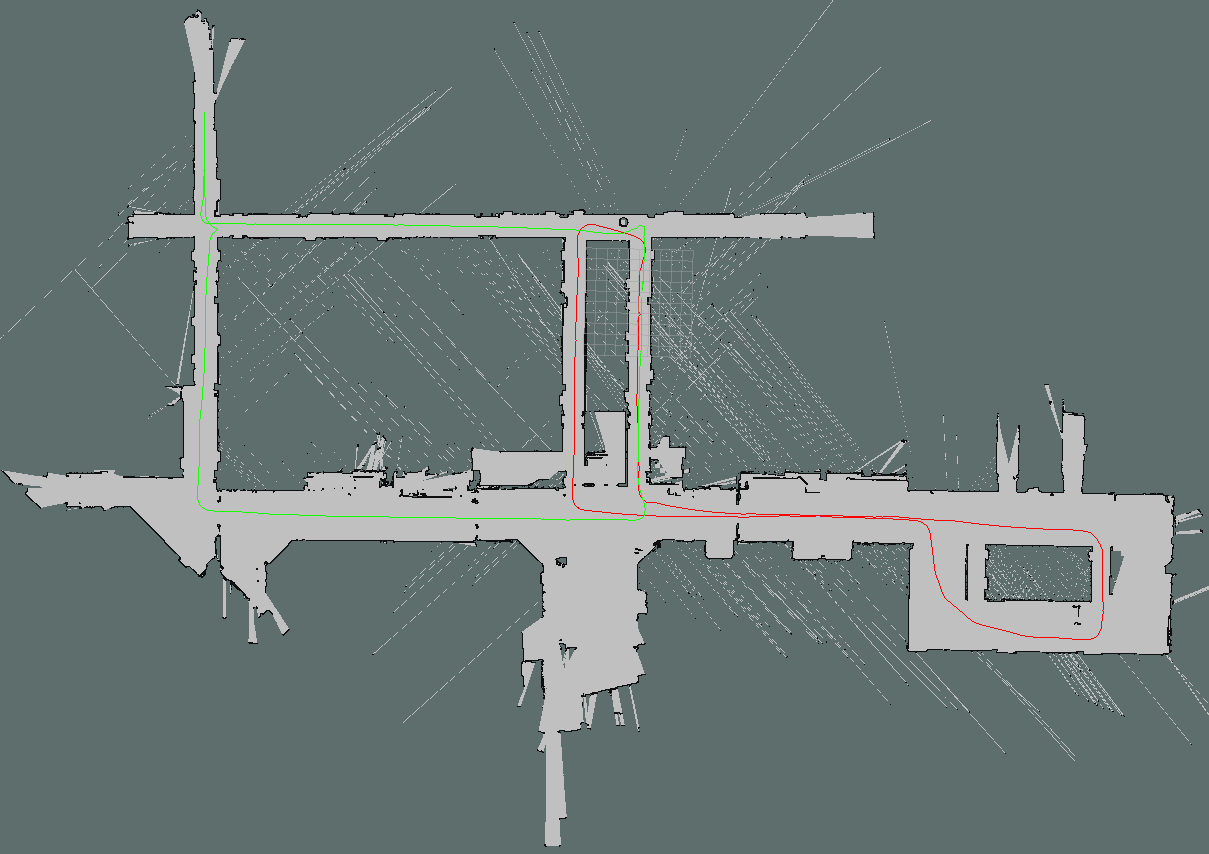
\includegraphics[width=0.9\textwidth]{img/multislam_big.png}
\end{center}
\caption{Mapping Example. Image depicts the resulting map of two cooperating robots. The red and green lines illustrate the estimated trajectory of both units. This map shows an additional feature of ohm\_tsd\_slam, the approach is able to map comparably large areas as the reconstructed map had an edge length of \unit[122]{m}. \textit{Source: Koch et. al.\cite{Koch2015}.}}
\label{fig:slam_map_expl}
\end{figure}


More information and a git repository regarding the 2D single or multi-SLAM ROS package ohm\_tsd\_slam can be found on the referring ROS Wiki page \cite{ohmtsdslam:ros}.

%what should come here:
%\todo{Phils part...}
%\begin{enumerate}
%	\item describe our slam algo
%	\item describe improvements from last robocup
%	\item picture from a map
%	\item refs to our tsd papers \cite{May2014}, \cite{Koch2015}
%	\item github source
%\end{enumerate}


\section{Localization}
As a first attempt on the RoboCup atWork \todo{consistent style of RaW} competition, we decided not to try the Precision Placement and Conveyor Belt test. It was a good idea because during this attempt we had big problems with the localization and navigation, which are basic functions. This limited us to try further and more difficult tests. We gain experience and improve our software so we will try this time more difficult tests.

We have three different strategies concerning the localization problem. The first one is to use our own particle filter algorithm. The second is to use the amcl package from ROS. And the third strategy is to use our SLAM algorithm mentioned in chapter~\ref{sec:slam} for localization. Because we have not yet decided which solution to use, we will mention all three in short.

\subsection{Particle-Filter (TH-Nuernberg)}
We are working on an own particle filter algorithm at our laboratory. Its functionality is close to amcl localization, \cite{pf_fox} and \cite{pr}. If we get it working in time, we would like to use our own software at the contest.

\subsection{Particle-Filter (ROS-AMCL)}
The navigation stack from ROS-System includes a package called amcl (adaptive Monte Carlo localization). It provides a particle filter algorithm for robot localization. We already checked the compatibility of amcl algorithm and our SLAM approach. So we are able to record a map with our SLAM algorithm and afterwards locate and navigate in that map via amcl and navigation stack from~ROS.

\subsection{SLAM for Localization}
SLAM means Simultaneous Localization and Mapping. This is because while recording a map, the robot needs to know its position in the map - so it must locate itself in the map while building the map. If we disable the mapping part from our SLAM algorithm, we are able to load a previously recorded map and locate the robot. The problem with this approach is that if the algorithm fails to process one measurement, the localization is lost in most cases and we have to quit the run. Particle filters are able to recover from such failures.

\todo{if we need more: multible laser scanner setup}


\section{Navigation}
%The data provided by the Hokuyo is additionally used for collision avoidance. If an obstacle is detected, a report goes to the path planning state which adjusts the path.
%
%There is no local navigation at the moment. In case we find an obstacle owr robot would stop and replan by using again the global navigation. We are thinking about implementing a second laser scaner and base the navigacion on the Slack\_navigation from ROS. Then we would also use a local navigation.

what should come here:
\begin{enumerate}
	\item describe navigation stack in short (we will use navigation from localization stack)
	\item describe problems and approach from last robocup\todo{jon}
\end{enumerate}

\section{Mission Planning}
For the main control of the system, a State Machine with singleton pattern design is used. Every state is designed to be as small as possible. For the German Open 2015, we implemented three main states divided on smaller sub-states: move, grasp and deliver.

Once we get the tasks from the referee box, the first step for every test is to drive to a specific position and an specific orientation. Once we are on the desired position we smoothly approach to the service area and perform the task of grasping or delivering an object. 	

\todo[noline]{statemachine image: use yed uml for statemachine and export it as nice cropped pdf}

\begin{figure}[htbp]
	\centering
	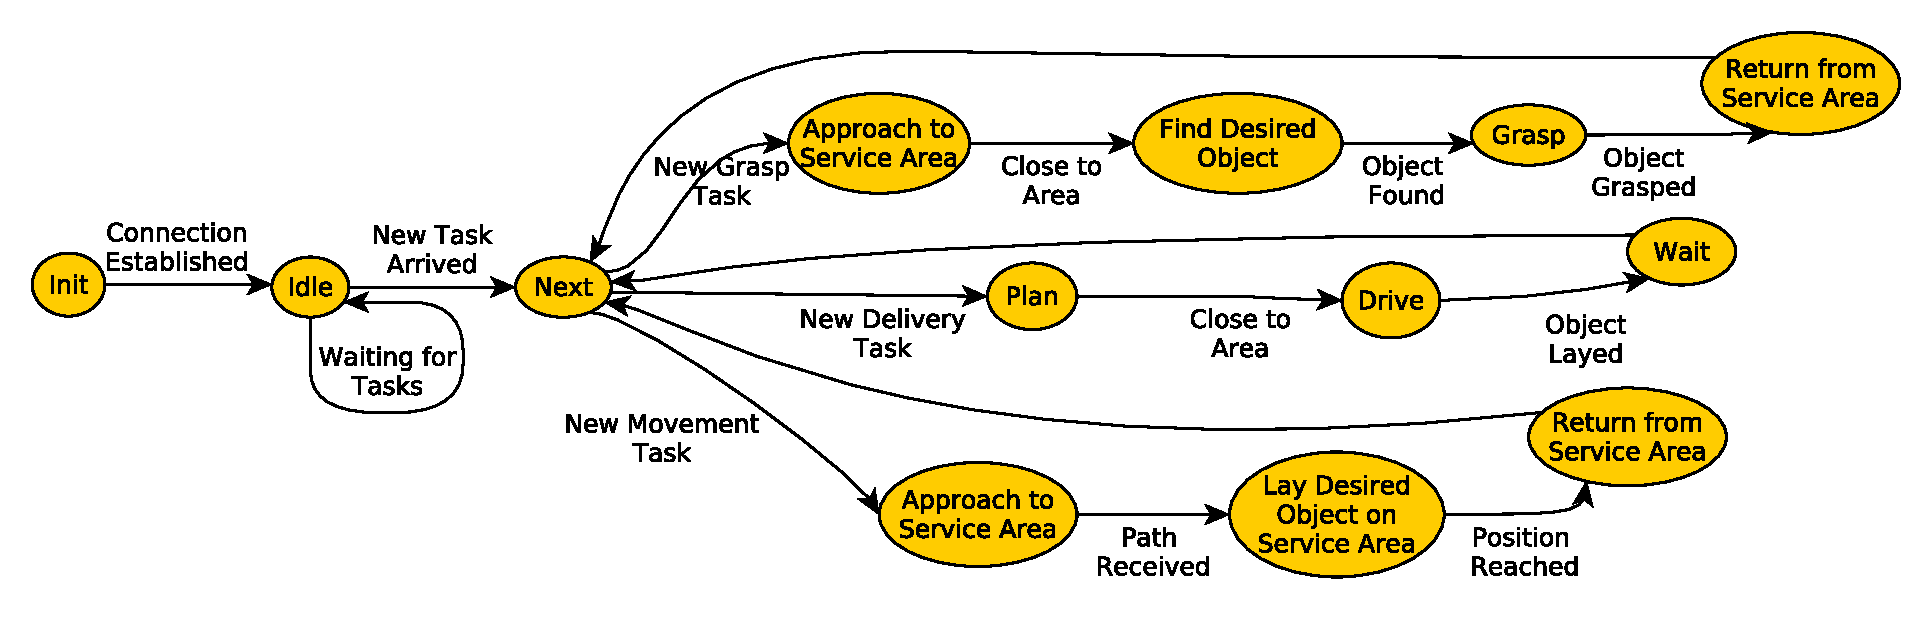
\includegraphics[width=\textwidth]{img/sm}
	\caption{Structure of the Statemachine}
	\label{fig:SM}
\end{figure}


The State Machine framework could be found on GitHub under our Laboratory's repository: "autonohm/obviously". 

\section{Object Manipulation}
To grasp objects reliably an exact position from the object perception is needed. The position of
objects will be calculated based on information, received from optical/infrared sensors (2D and 3D).
After the calculation is finished the robot will navigate to a pregrasp position. Once the base has
reached the final position, kinematics will lead the arm near the object. For precise gripping a
2D/3D optical/infrared sensor has been attached to the end effector. In gripping stance the arm-
2camera will be activated to measure the final gripping pose. Because manipulation is an upcoming
issue in our robotic institute, a self developed inverse kinematic is deployed.
%we decided to build our own inverse kinematic.

\section{Conclusion}
In this paper we first briefly introduce our Autonohm \todo{consistent writing} team and team members. We then present the HW we use and give a brief explanation about the SW packages we are using. We also describe more in detail the software developed by us such as the 2D image processing software, mapping, localization and state machine. \todo{we also 2x}

\end{document}
